\documentclass{article}
\usepackage[utf8]{inputenc}
\usepackage[T1]{fontenc}
\usepackage[english]{babel}
\setlength{\parindent}{0pt}
\usepackage{hyperref}
\hypersetup{
    colorlinks=true,
    linkcolor=blue,
    filecolor=magenta,      
    urlcolor=cyan}
\usepackage{graphicx}
\graphicspath{ {./pic/} }
\usepackage{fourier,amssymb,microtype,amsmath,gensymb}
\newcommand{\R}{\mathbb{R}}
\usepackage{mdframed,caption,xcolor,enumitem}
\usepackage{tikz,tkz-euclide}

\title{Seminar 2 - Expenditure function \& Substitution effects}
\author{Xiaoguang Ling \\  \href{xiaoguang.ling@econ.uio.no}{xiaoguang.ling@econ.uio.no}}
\date{\today}

\begin{document}

\maketitle

%%%%%%%%%%%%%%%%%%%%%%%%%%%%%%%%%%%%%%%%%%%%%%%%%%%%%%%%%%%%%%%%%%%%%%%%%%%%%%%%%%%%%%%%%%%%%%
\section{Jehle \& Reny 1.38 - Properties of the Expenditure Function}
Verify that the expenditure function obtained from the CES direct utility function in Example 1.3 
(JR. pp.39) satisfies all the properties given in Theorem 1.7 (JR. pp.37).

\begin{mdframed}[backgroundcolor=blue!20,linecolor=white]

\textbf{Expenditure Function (JR. pp.35)}

\medskip

We define the expenditure function as the minimum-value function:

$$e(p, u) \equiv \min_{x \in \R^n_+} p \cdot x$$

\textbf{Expenditure Function of CES direct utility function (JR. pp.39)}

\medskip

In Example 1.3 (JR. pp.39), we have a so called CES  direct utility function:
$$u(x_1, x_2) = (x_1^{\rho} + x_2^{\rho})^{\frac{1}{\rho}},\ where \ 0 \ne \rho<1.$$

To derive the Expenditure Function, we need to solve the expenditure minimisation problem
given some utility $u$. i.e.
$$\min_{x_1,x_2} \ p_1x_1 + p_2x_2 \ \ s.t.  \ \ u(x_1, x_2) = (x_1^{\rho} + x_2^{\rho})^{\frac{1}{\rho}} = u, \ x_1 \ge 0, \ x_2 \ge 0$$

(Read JR. pp.40 to see how to minimize the expenditure with Lagrangian method.)

\medskip

The solution to the expenditure-minimisation problem is called the consumer’s
vector of \textbf{Hicksian demands}:

\begin{equation}
    \begin{cases}
    x_1^h(p_1,p_2,u) = u(p_1^{r} + p_2^{r})^{\frac{1}{r}-1} p_1^{(r-1)} \\	
    x_1^h(p_1,p_2,u) = u(p_1^{r} + p_2^{r})^{\frac{1}{r}-1} p_2^{(r-1)} \\	
    \end{cases}
    \label{eq:1_38_hicks}   
\end{equation}

Here $r \equiv \frac{\rho}{\rho - 1}$.

Substitute the solution above (Equation \ref{eq:1_38_hicks}) into our
objective function  $p_1x_1 + p_2x_2$ to obtain the Expenditure Function:

$$e(p_1,p_2, u) = p_1x_1^h(p_1,p_2,u) + p_2x_2^h(p_1,p_2,u) = 
u(p_1^{r} + p_2^{r})^{\frac{1}{r}} , r \equiv \frac{\rho}{\rho - 1}$$

\textbf{THEOREM 1.7 Properties of the Expenditure Function (JR. pp.37)}

\medskip

If $u(.)$ is continuous and strictly increasing, then $e(p, u)$ defined in (1.14) is

\begin{enumerate}
\item Zero when $u$ takes on the lowest level of utility in $\mathcal{U}$,
\item Continuous on its domain $\R^n_{++} \times \mathcal{U}$,
\item For all $p \gg 0$, strictly increasing in $u$ and unbounded above in $u$,
\item Increasing in $p$,
\item Homogeneous of degree $1$ in $p$,
\item Concave in $p$.
\end{enumerate}
If, in addition, $u(.)$ is strictly quasiconcave, we have
\begin{enumerate}[start = 7]
\item Shephard’s lemma: $e(p, u)$ is differentiable in $p$ at $(p^0, u^0)$ with $p^0 \gg 0$, and
$$\frac{\partial e(p^0, u^0)}{\partial p_i} = x^h_i (p^0, u^0), \ \ \ \ i = 1, . . . , n.$$
\end{enumerate}
\end{mdframed}

Firstly we should know that the CES direct utility function $u(x_1, x_2) = (x_1^{\rho} + x_2^{\rho})^{\frac{1}{\rho}},\ where \ 0 \ne \rho<1.$ is continuous and strictly increasing (can be proved similarly as below), which is the
prerequisite of Theorem 1.7.

%***************************************************
\subsection{$e(p, u)$ is zero when $u$ takes on the lowest level of utility in $\mathcal{U}$}
\begin{mdframed}[backgroundcolor=blue!20,linecolor=white]
\textit{"no consumption, no expenditure"}

\end{mdframed}


As usual, we assume non-negative consumption, i.e. $x \in R^n_+$. Since $u(.)$ is strictly increasing,
$u_{min} = u(0,0) = 0$. 

When $u = 0$, we have $e(p,0) = 0 \times (p_1^{r} + p_2^{r})^{\frac{1}{r}} =0$.


%***************************************************
\subsection{$e(p, u)$ is continuous on its domain $\R^n_{++} \times \mathcal{U}$,}


\begin{mdframed}[backgroundcolor=blue!20,linecolor=white]
We want a function to be continuously differentiable because we can then take derivatives (to study its property) freely.

For a ONE dimention function $f(x)$, if the derivative at $x = a$ (i.e. $f'(a)$) exists, it's differentiable at $x = a$.
$\Rightarrow f(x)$ is continuous at $x = a$.

For a higher dimension function, the existance of all partial/directional derivatives is not
sufficient for its differentiability. Here are examples from Wikipedia: \href{https://en.wikipedia.org/wiki/Differentiable_function}{Differentiability in higher dimensions}

$e(p_1,p_2,u)$ is a 3-dimension function. If you really want to prove it's differentiable ($\Rightarrow$ continuous), you can either try to use the definition of differentiable functions. You can also read theorem A2.21 (Jehle \& Reny pp.602) and theorem 1.9 (point 3,Jehle \& Reny  pp.520).
\end{mdframed}

\begin{mdframed}[backgroundcolor=yellow!20,linecolor=white]
Good news for your exam:

\textit{"There is no need to prove continuity (or concavity) of higher dimension functions (in your exam). I might ask you to prove continuity (or concavity) wrt one variable (a specific price, for example)." -- Paolo}
\end{mdframed}



For this sub-question, let's assume the prices are given (say, by the market). Therefore
$e(p_1,p_2,u) = e(u)$ is one dimesional.

Obviously, $$\frac{d e(u)}{d u} = \frac{d u(p_1^{r} + p_2^{r})^{\frac{1}{r}} }{d u} = (p_1^{r} + p_2^{r})^{\frac{1}{r}}$$

The derivetive exists for any $u \in \mathcal{U}$. $e(u)$ is differentiable and thus continuous.


%***************************************************
\subsection{For all $p \gg 0$, $e(p, u)$ is strictly increasing in $u$ and unbounded above in $u$,}
\begin{mdframed}[backgroundcolor=blue!20,linecolor=white]
\textit{"more utility, more expenditure"}

\end{mdframed}


Since $\frac{d e(u)}{d u} = (p_1^{r} + p_2^{r})^{\frac{1}{r}} > 0, \forall p \gg 0$,
$e(p_1,p_2,u)$ is strictly increasing in $u$.

Given the positive prices, $\lim_{u\to\infty} e(u) = \lim_{u\to\infty} u(p_1^{r} + p_2^{r})^{\frac{1}{r}}= + \infty$. It there is no upper boundary in $u$.


%***************************************************
\subsection{$e(p, u)$ is increasing in $p$,}

$$\frac{\partial e(p_1,p_2, u)}{\partial p_1} = \frac{\partial u(p_1^{r} + p_2^{r})^{\frac{1}{r}} }{\partial p_1} = u \cdot \frac{1}{r}(p_1^{r} + p_2^{r})^{\frac{1}{r} - 1} \cdot r  p_1^{r-1} =
u (p_1^{r} + p_2^{r})^{\frac{1}{r} - 1} p_1^{r-1} > 0$$

$$\frac{\partial e(p_1,p_2, u)}{\partial p_2} = \frac{\partial u(p_1^{r} + p_2^{r})^{\frac{1}{r}} }{\partial p_2} = u \cdot \frac{1}{r}(p_1^{r} + p_2^{r})^{\frac{1}{r} - 1} \cdot r  p_2^{r-1} =
u (p_1^{r} + p_2^{r})^{\frac{1}{r} - 1} p_2^{r-1} > 0$$

Therefore $e(p, u)$ is increasing in $p$.


%***************************************************
\subsection{$e(p, u)$ is homogeneous of degree $1$ in $p$,}

\begin{mdframed}[backgroundcolor=blue!20,linecolor=white]

\textit{"Inflation"}

Homogeneous functions (Jehle \& Reny Definition A2.2 pp.561):

$f(x)$ is called homogeneous of degree $k$ if $f(tx) \equiv t^kf(x),\ \forall t > 0$

You want to show $e(tp, u) = t^1e(p, u),\ \forall t > 0$
\end{mdframed}

For any $t>0$,

\begin{align*}
e(u,tp) &= u[(tp_1)^{r} + (tp_2)^{r}]^{\frac{1}{r}} \\
&= u[t^r(p_1^{r} + p_2^{r})]^{\frac{1}{r}} \\
&= tu(p_1^{r} + p_2^{r})^{\frac{1}{r}} \\
&= t^1e(u,p)
\end{align*}

Therefore $e(p, u)$ is homogeneous of degree $1$ in $p$.

%***************************************************
\subsection{$e(p, u)$ is concave in $p$.}


\begin{mdframed}[backgroundcolor=yellow!20,linecolor=white]
\begin{itemize}
\item In exam one-dimension function is most common, which means you only need to 
calculate its second derivative to prove concavity.

\item Before you prove it, think about the intuition of the curve (function). Diminishing
marginal effects is very common in economics, which also implies concavity. 

\item Do NOT prove anything if the question doesn't require you. Just answer yes or no if the question
simply asks "Is the function concave? Is it increasing? etc."
\end{itemize}
\end{mdframed}

\begin{mdframed}[backgroundcolor=blue!20,linecolor=white]

\textit{"Diminishing marginal expenditure (in $p$)"}

Concave functions (Jehle \& Reny pp.534):

$f : D \to \R \ $ is a concave function if for all $x^1, x^2 \in D$,

$$f(x^t) \ge tf(x^1) + (1 − t)f(x^2), \ \forall t \in [0, 1].$$

Where $x^t \equiv tx^1 + (1-t)x^2, t \in [0,1].$

\vspace{2mm}
{\centering
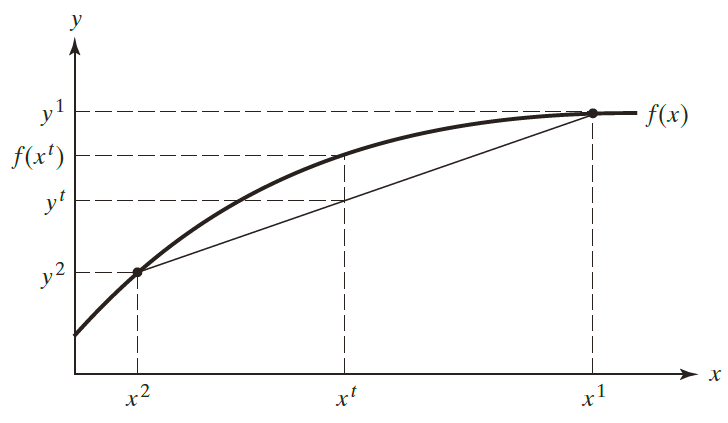
\includegraphics[width=0.8\textwidth]{2.concavef}
\captionof{figure}{Concave functions}
\label{cf}}
\vspace{2mm}


\begin{itemize}
\item Intuition: $e(p,u)$ is increasing \textbf{in $p$} but the marginal expenditure is diminishing.
\end{itemize}

For this specific function $e(p_1,p_2,u)$, you can follow the very smart proof on Jehle \& Reny pp. 38-39 to show that for any given utility $\bar{u}$, $$e[tp^1+(1-t)p^2,\bar{u}] \ge te(p^1,\bar{u}) + (1-t)e(p^2,\bar{u})$$

Where $p^1 = \left(\begin{smallmatrix}p^1_1 \\ p^1_2\end{smallmatrix}\right)$ and $p^2 = \left(\begin{smallmatrix}p^2_1 \\ p^2_2\end{smallmatrix}\right)$ are two price sets. $t \in [0,1]$

\vspace{2mm}


\textbf{We can also prove it's concavity using derivatives.} 

\vspace{2mm}

\textbf{For a (twice differentiable) one-dimension function $f(x)$ with diminishing margin (
concave towards x-axis), $f''(x)<0$, i.e.}
$$f(x) \ is \  concave \iff f''(x) < 0$$

\noindent\makebox[\linewidth]{\rule{12cm}{0.4pt}}

\vspace{2mm}

(Read the following creteria and proof if you're interested)

\vspace{2mm}

For a higher dimension function $e(p_1,p_2,u)$, it's natural to think about how the derivatives look like.


\vspace{2mm}

We call the second derivatives of a n-demension function $f$ "\textbf{Hessian matrix}" ($H(x)$, Jehle \& Reny pp.557):

\begin{equation}
H(x)=\left(
    \begin{array}{cccc}
		f_{11}(x) & f_{12}(x) & \cdots & f_{1n}(x) \\
		f_{21}(x) & f_{22}(x) & \cdots & f_{2n}(x) \\
		\vdots    &    \vdots & \ddots &   \vdots \\
		f_{n1}(x) & f_{n2}(x) & \cdots & f_{nn}(x) \\
    \end{array}
    \right)
\label{eq:hessian}   
\end{equation}

\vspace{2mm}

We can use the following facts about $H(x)$ and concavity(\href{https://mjo.osborne.economics.utoronto.ca/index.php/tutorial/index/1/qfs/t\#:~:text=Finally\%2C\%20the\%20matrix\%20has\%20one,namely\%20its\%20determinant\%2C\%20\%E2\%88\%9219.&text=A\%20is\%20positive\%20semidefinite\%20if,and\%20nonnegative\%20for\%20k\%20even.}{More details and examples}):

\begin{itemize}
\item  \textbf{Theorem A2.4}(Jehle \& Reny pp.559): If function $f$ is twice continuously differentiable on a convex open set $S$, then 
$f$ is concave $\iff$ the Hessian matrix $H(x)$ of $f$ is \href{https://towardsdatascience.com/what-is-a-positive-definite-matrix-181e24085abd}{negative semidefinite} for all $x \in S$

\item \textbf{Negative semidefinite}(Jehle \& Reny pp.559): a $n \times n$ metrix $H$ is negative semidefinite $\iff \ H$'s $k$th order principal minors are nonpositive for $k$ odd and nonnegative for $k$ even.

\item The $k$th order principal minors of an $n \times n$ symmetric matrix $H$ are the determinants of the $k \times k$ matrices obtained by deleting $n − k$ rows and the corresponding $n − k$ columns of $H$ (where $k = 1, ..., n$).

\end{itemize}

\vspace{2mm}

The Hessian matrix of $e(p_1,p_2,u)$ (in $p$) is:

\vspace{2mm}


\begin{equation}
H(p)=\left(
    \begin{array}{cc}
		e_{p_1p_1} & e_{p_1p_2}  \\
		e_{p_2p_1} & e_{p_2p_2}  \\
    \end{array}
    \right) 
\label{eq:hessian_e}   
\end{equation}

\vspace{2mm}

$H(p)$ contains two 1st order ($k = 1, n - k = 2 -1 = 1$) principal minors: $e_{p_1p_1}$ and $e_{p_2p_2}$, and one 2nd order ($k = 2, n - k = 2 -2 = 0$) principal minors:
\begin{equation}
    \begin{vmatrix}
		e_{p_1p_1} & e_{p_1p_2}  \\
		e_{p_2p_1} & e_{p_2p_2}  \\
    \end{vmatrix}
=e_{p_1p_1}e_{p_2p_2} - e_{p_1p_2}e_{p_2p_1}
\label{eq:pminor_e}   
\end{equation}

We want to prove:

\begin{itemize}
\item  $e_{p_1p_1} \le 0$  and $e_{p_2p_2} \le 0$
\item  $e_{p_1p_1}e_{p_2p_2} - e_{p_1p_2}e_{p_2p_1} \ge 0$

\end{itemize}

We already know $\frac{\partial e(p_1,p_2)}{\partial p_1} =
u (p_1^{r} + p_2^{r})^{\frac{1}{r} - 1} p_1^{r-1}$, and 
$\frac{\partial e(p_1,p_2)}{\partial p_2} = 
u (p_1^{r} + p_2^{r})^{\frac{1}{r} - 1} p_2^{r-1}$


\begin{align*}
\frac{\partial e(p_1,p_2)}{\partial p_1\partial p_1} &=
\frac{\partial u (p_1^{r} + p_2^{r})^{\frac{1}{r} - 1} p_1^{r-1}}{\partial p_1} \\
&= u (\frac{1}{r} - 1)(p_1^{r} + p_2^{r})^{\frac{1}{r} - 2}rp_1^{r-1}p_1^{r-1} + u(p_1^{r} + p_2^{r})^{\frac{1}{r} - 1}(r-1)p_1^{r-2} \\
&= u(p_1^{r} + p_2^{r})^{\frac{1}{r} - 1} p_1^{r-2}[(\frac{1}{r} - 1)(p_1^{r} + p_2^{r})^{-1}rp_1^{r} + (r-1)] \\
&= u(p_1^{r} + p_2^{r})^{\frac{1}{r} - 1} p_1^{r-2} (1-r)[\frac{p_1^{r}}{(p_1^{r} + p_2^{r})} - 1] \\
&= u(p_1^{r} + p_2^{r})^{\frac{1}{r} - 2} p_1^{r-2} (r-1)p_2^r \\
\end{align*}

\begin{equation}
\because \ \ \
    \begin{cases}
u(p_1^{r} + p_2^{r})^{\frac{1}{r} - 2} p_1^{r-2}p_2^r \ge 0 \\
r \equiv \frac{\rho}{\rho - 1} = \frac{1}{1 - \frac{1}{\rho}} < 1, \forall \rho < 1, \rho \ne 0 \Rightarrow r-1 \le 0 \\
    \end{cases}
\nonumber
\end{equation}

$\therefore e_{p_1p_1} \le 0$

Similarly, $e_{p_2p_2} = u(p_1^{r} + p_2^{r})^{\frac{1}{r} - 2} p_2^{r-2} (r-1)p_1^r \le 0$ (note $p_1$ and $p_2$ are "symmetric").

\begin{align*}
\frac{\partial e(p_1,p_2)}{\partial p_1\partial p_2} &=
\frac{\partial u (p_1^{r} + p_2^{r})^{\frac{1}{r} - 1} p_1^{r-1}}{\partial p_2} \\
&= u ({\frac{1}{r} - 1})(p_1^{r} + p_2^{r})^{\frac{1}{r} - 2} rp_2^{r-1}p_1^{r-1} \\
&= u (1-r)(p_1^{r} + p_2^{r})^{\frac{1}{r} - 2} p_2^{r-1}p_1^{r-1} \\
\end{align*}

According to Young's theorem (Jehle \& Reny pp.557),$\frac{\partial e(p_1,p_2)}{\partial p_1\partial p_2} = \frac{\partial e(p_1,p_2)}{\partial p_2\partial p_1}$ 

We have
\begin{align*}
&e_{p_1p_1}e_{p_2p_2} - e_{p_1p_2}e_{p_2p_1} \\
&=[u(p_1^{r} + p_2^{r})^{\frac{1}{r} - 2} p_1^{r-2} (r-1)p_2^r][u(p_1^{r} + p_2^{r})^{\frac{1}{r} - 2} p_2^{r-2} (r-1)p_1^r] \\
& - [u (1-r)(p_1^{r} + p_2^{r})^{\frac{1}{r} - 2} p_2^{r-1}p_1^{r-1}]^2 \\ &=u^2(p_1^{r} + p_2^{r})^{\frac{2}{r} - 4}(p_1p_2)^{2r-2)} (r-1)^2 -
u^2(1-r)^2(p_1^{r} + p_2^{r})^{\frac{2}{r} - 4} (p_2p_1)^{2r-2} \\
&= 0 \ge 0
\end{align*}

Therefore, $H(p)$ is negative semidefinite $\Rightarrow \ e(p,u)$ is concave in $p$.

\end{mdframed}

%***************************************************
\subsection{If $u(.)$ is also strictly quasiconcave, we have Shephard’s lemma: $e(p, u)$ is differentiable in $p$ at $(p^0, u^0)$ with $p^0 \gg 0$, and $\frac{\partial e(p^0, u^0)}{\partial p_i} = x^h_i (p^0, u^0), \ \ \ \ i = 1, . . . , n$.}

\begin{mdframed}[backgroundcolor=blue!20,linecolor=white]
\textit{"Compensated demands"}

Again, the proof for $e(p,u)$ is differentiable at $(p^0,u^0)$ in $p$ with $p^0 \gg 0$ is not required by our course.

CES utility function $u(x_1, x_2) = (x_1^{\rho} + x_2^{\rho})^{\frac{1}{\rho}}, \ 0 \ne \rho<1.$ has a similar form as the expenditure function 
$e(p_1,p_2, u) = u(p_1^{r} + p_2^{r})^{\frac{1}{r}} , r \equiv \frac{\rho}{\rho - 1}$. You can similarly prove it is concave ($\Rightarrow$ quasiconcave, see also Thorem A1.15 on Jehle \& Reny pp. 541).

\vspace{3mm}

\textbf{Shephard’s lemma} states the fact that the Hicksian demands on $x_i=$ the partial derivatives of the expenditure functions on $p_i$.

\textbf{Intuition:} Hicksian demands are also called "compensated demands": given utility $\bar{u}$, when price $p_i$ changed a little, how your demand will change to achieve the same utility level $\bar{u}$?

\end{mdframed}


$$\frac{\partial e(p_1,p_2)}{\partial p_1} =
u (p_1^{r} + p_2^{r})^{\frac{1}{r} - 1} p_1^{r-1}$$

$$\frac{\partial e(p_1,p_2)}{\partial p_2} = 
u (p_1^{r} + p_2^{r})^{\frac{1}{r} - 1} p_2^{r-1}$$

Compare these derivatives with the Hicksian demand in Equation \ref{eq:1_38_hicks}.


%%%%%%%%%%%%%%%%%%%%%%%%%%%%%%%%%%%%%%%%%%%%%%%%%%%%%%%%%%%%%%%%%%%%%%%%%%%%%%%%%%%%%%%%%%%%%%
\section{Jehle \& Reny 1.44 - Inferior and Normal goods}
In a two-good case, show that if one good is inferior, the other good must be normal.

\begin{mdframed}[backgroundcolor=blue!20,linecolor=white]
The question is actually based on the assumption that $u(.)$ is strictly increasing. Therefore you will always use your budget up to maximize your utility ( $p_1x_1 + p_2x_2 = y$). This is called "Budget Balancedness"(Theorem 1.10 on Jehle \& Reny pp. 49).

\end{mdframed}

Assume there are only 2 goods , $x_1, x_2 \in \R^2_+$, the price vector
$p' = (p_1,p_2) \gg 0$, $y$ is the income and the budget constraint is $p_1x_1 + p_2x_2 \le y$.

We always assume u(.) is strictly increasing, therefore we have budget balancedness to maximize the utility:$p_1x_1 + p_2x_2 = y$

If $x_1$ is inferior, it means the demand for $x_1$ will decrease when the income increases, i.e. $\frac{\partial x_1(p_1,p_2,y)}{\partial y} < 0$.

If $x_2$ is also inferior, what will happen when $y$ increases? The left-hand side will decrease but the right-hand side will increase, which is impossible. Therefore  $x_2$ must be normal.

\begin{mdframed}[backgroundcolor=blue!20,linecolor=white]
You can also take derivatives on both sides of the budget balancedness to avoid wordy argument:

\begin{align*}
\frac{\partial (p_1x_1 + p_2x_2)}{\partial y} &= \frac{dy}{dy} \\
p_1\frac{\partial x_1}{\partial y} + p_2\frac{\partial x_2}{\partial y} &= 1 \\
\frac{\partial x_2}{\partial y} &= \frac{1}{p_2}
(1- p_1\frac{\partial x_1}{\partial y}) >0 \\
\end{align*}
\end{mdframed}

%%%%%%%%%%%%%%%%%%%%%%%%%%%%%%%%%%%%%%%%%%%%%%%%%%%%%%%%%%%%%%%%%%%%%%%%%%%%%%%%%%%%%%%%%%%%%%
\section{Jehle \& Reny 1.51 - Substitues and Complements}
Consider the utility function, $u(x_1, x_2) = (x_1)^{1/2} + (x_2)^{1/2}$.

\begin{enumerate}[label=\alph*.]

\item Compute the demand functions, $x_i(p_1, p_2, y), \ i = 1, 2$.

\item Compute the substitution term in the Slutsky equation for the effects on $x_1$ of changes in $p_2$.

\item Classify $x_1$ and $x_2$ as (gross) complements or substitutes.

\end{enumerate}

%***************************************************
\subsection{Compute the demand functions, $x_i(p_1, p_2, y), \ i = 1, 2$}

\begin{mdframed}[backgroundcolor=blue!20,linecolor=white]
Marshallian demand functions $x^* = x(p, y)$ is the solutions 
to the utility maximization problem (JR. pp.21).
\end{mdframed}

There is no corner solution:

\begin{itemize}
\item The function is strictly increasing so the budget balancedness holds. 
\item The marginal utility $u_{x_1} = 0.5x_1^{-0.5}$ and $u_{x_2} = 0.5x_2^{-0.5}$ go to infinite as $x_i \to 0$, constraints $x_1 \ge 0$  and  $x_2 \ge 0$ can not be binding. 
\end{itemize}


\begin{mdframed}[backgroundcolor=yellow!20,linecolor=white]
In exam, always discuss if interior solutions exist, in case you make mistakes! Especially when you get weired object functions or contradictory results.

(Compare this question with Jehle \& Reny 1.26.)
\end{mdframed}


We want to solve the utility maximization problem with some $(x_1^*, x_2^*)$, i.e.
$$\max_{x_1,x_2} \ u(x_1,x_2) = x_1^{0.5} + x_2^{0.5} \ \ s.t. \ p_1x_1 + p_2x_2 = y$$


Lagrangean: $$L = x_1^{0.5} + x_2^{0.5} + \lambda (y - p_1x_1 -p_2x_2)$$
FOCs:
\begin{equation}
\begin{cases}
\frac{\partial L}{\partial x_1} &= 0.5x_1^{-0.5} -p_1\lambda = 0 \\
\frac{\partial L}{\partial x_2} &= 0.5x_2^{-0.5} -p_2\lambda = 0 \\
\frac{\partial L}{\partial \lambda} &= y - p_1x_1 -p_2x_2 =0
\end{cases}
\nonumber
\end{equation}

Simplify:

\begin{equation}
\begin{cases}
0.5x_1^{-0.5} &= p_1\lambda \\
0.5x_2^{-0.5} &= p_2\lambda \\
p_1x_1 + p_2x_2 &= y
\end{cases}
\end{equation}

Take the ratio between first and second condition to get:
$$(\frac{x_1}{x_2})^{-0.5} = \frac{p_1}{p_2} \Rightarrow x_1 = (\frac{p_1}{p_2})^{-2}x_2 $$
Substitute $x_1$ with $x_2$ in the 3rd condition to get:

$$p_1(\frac{p_1}{p_2})^{-2}x_2 + p_2x_2 = y$$ 

$$\Rightarrow x_2 = \frac{y}{p_1(\frac{p_1}{p_2})^{-2} + p_2} = \frac{y}{p_1(\frac{p_2^2}{p_1^2}) + p_2} =\frac{p_1y}{p_2^2 + p_1p_2} = \frac{p_1}{p_2}\frac{y}{p_1 + p_2}$$

Thus:
$$x_1 = (\frac{p_1}{p_2})^{-2}x_2 = (\frac{p_1}{p_2})^{-2}\frac{p_1}{p_2}\frac{y}{p_1 + p_2} =\frac{p_2}{p_1}\frac{y}{p_1 + p_2}$$


\begin{mdframed}[backgroundcolor=blue!20,linecolor=white]
Since there are only 2 variables $x_1$ and $x_2$ in your object function
$u(x_1,x_2)$ and you already know the budget must be binding, i.e.
$y = p_1x_1 + p_2x_2$, you can actually transform $u(x_1,x_2)$  into 
a function of only $x_1$ or $x_2$:

$$y = p_1x_1 + p_2x_2 \Rightarrow x_1 = \frac{y-p_2x_2}{p_1}$$

$$u(x_1,x_2)= x_1^{0.5} + x_2^{0.5} = (\frac{y-p_2x_2}{p_1})^{0.5} + x_2^{0.5}$$

Since the question ask you to maximize $u(x_1,x_2)$, if you solve $\frac{d u(x_2)}{d x_2} = 0$ and get only one solution, it is the solution.


\begin{align*}
\frac{d u(x_2)}{d x_2} = 0.5[ (\frac{y-p_2x_2}{p_1})^{-0.5}](\frac{-p_2}{p_1}) + 0.5x_2^{-0.5} &= 0 \\
(\frac{y-p_2x_2}{p_1})^{-0.5}\frac{p_2}{p_1} &= x_2^{-0.5} \\
\frac{y-p_2x_2}{p_1}\frac{p_2^{-2}}{p_1^{-2}} &= x_2 \\
\frac{y-p_2x_2}{p_1}\frac{p_1^{2}}{p_2^{2}} &= x_2 \\
y\frac{p_1}{p_2^{2}} - \frac{p_1}{p_2}x_2&= x_2 \\
x_2 + \frac{p_1}{p_2}x_2 &=  y\frac{p_1}{p_2^{2}} -\\
x_2 &=  \frac{1}{1+\frac{p_1}{p_2}}y\frac{p_1}{p_2^{2}} \\
x_2 &=  \frac{p_1}{p_2}\frac{y}{p_1 + p_2}
\end{align*}

You then solve $x_1$ with the budget constraint
\end{mdframed}


%***************************************************
\subsection{Compute the substitution term in the Slutsky equation for the effects on $x_1$ of changes in $p_2$}

\begin{mdframed}[backgroundcolor=blue!20,linecolor=white]
\textbf{THEOREM 1.11 Slutsky equation}(Jehle \& Reny pp.53)

Let $x(p, y)$ be the consumer’s Marshallian demand system. Let $u^*$ be the level of utility the consumer achieves at prices $p$ and income $y$. Then,
$$\underbrace{\frac{\partial x_i(p,y)}{\partial p_j}}_{TE} = \underbrace{\frac{\partial x_i^h(p,u^*)}{\partial p_j}}_{SE} \underbrace{- x_j(p,y)\frac{\partial x_i(p,y)}{\partial y}}_{IE} , \  i,j = 1,2,...,n.$$

Slutsky equation decomposes the change of demand when price changes (TE) into
2 parts: substitution effects (SE) and income effects (IE).

The question asks you to compute SE, and you already have Marshallian demand function in question part (a), it's easier to use $SE = TE + IE$ directely

\end{mdframed}

\begin{align*}
\frac{\partial x_1^h(p,u^*)}{\partial p_2} &= \frac{\partial x_1(p,y)}{\partial p_2} + x_2(p,y)\frac{\partial x_1(p,y)}{\partial y} \\
&= \frac{\partial (\frac{p_2}{p_1}\frac{y}{p_1 + p_2})}{\partial p_2} + (\frac{p_1}{p_2}\frac{y}{p_1 + p_2})\frac{\partial (\frac{p_2}{p_1}\frac{y}{p_1 + p_2})}{\partial y} \\
&= \frac{1}{p_1}\frac{y}{p_1 + p_2} + \frac{p_2}{p_1}\frac{-y}{(p_1 + p_2)^2} + (\frac{p_1}{p_2}\frac{y}{p_1 + p_2})(\frac{p_2}{p_1}\frac{1}{p_1 + p_2}) \\
&=\frac{\frac{(p_1+p_2)}{p_1} y}{(p_1 + p_2)^2} - \frac{\frac{p_2}{p_1}y}{(p_1 + p_2)^2} +\frac{y}{(p_1 + p_2)^2} \\
&=\frac{2y}{(p_1 + p_2)^2} 
\end{align*}

%***************************************************
\subsection{Classify $x_1$ and $x_2$ as (gross) complements or substitutes}

\begin{mdframed}[backgroundcolor=blue!20,linecolor=white]

How to define complements and substitutes? If $\frac{\partial x_b}{\partial p_a} > 0$, are $x_a,x_b$ substitutes?

Here is an example:

\begin{itemize}
\item As fruits, apple and banana seems to be "substitutes", i.e. when apple price increases, we tend to buy fewer apples and more bananas($\frac{\partial x_b}{\partial p_a} > 0$).

\item However, since apples are very expensive, ony a few apples cost so much money that you have less money for bananas. As a result, you buy fewer apples and fewer bananas ($\frac{\partial x_b}{\partial p_a} < 0$).

\item Things get more complex when banana is inferior, which leads to a positive income effect when apple price increase. 
\end{itemize}

\begin{center}
\textbf{Substitute effects may be "covered" by the income effects}
\end{center}


To precisely describe "substitutes" we need to define:

\begin{itemize}
\item Gross substitutes: $\frac{\partial x_b}{\partial p_a} > 0$
\item Net substitutes: $\frac{\partial x^h_b(\bar{u})}{\partial p_a} > 0$
\end{itemize}

\end{mdframed}

Since $\frac{\partial x_1^h(p,u^*)}{\partial p_2} = \frac{2y}{(p_1 + p_2)^2}>0$, we already know $x_1, x_2$ are net substitutes.

$$\frac{\partial x_1(p,y)}{\partial p_2} = \frac{\partial (\frac{p_2}{p_1}\frac{y}{p_1 + p_2})}{\partial p_2} = \frac{1}{p_1}\frac{y}{p_1 + p_2} > 0$$

$\Rightarrow x_1, x_2$ are also gross substitutes

\end{document}